\documentclass[10pt,a4paper]{article}
\usepackage[utf8]{inputenc}
\usepackage[spanish]{babel}
\usepackage{amsmath}
\usepackage{amsfonts}
\usepackage{amssymb}
\usepackage{makeidx}
\usepackage{graphicx}
\usepackage{lmodern}
\graphicspath{{imagenes/}}	
\usepackage[left=2cm,right=2cm,top=2cm,bottom=2cm]{geometry}
\author{Sistemas evolutivos\\INAOE\\Ciro Fabian Bermudez Marquez\\cirofabian.bermudez@gmail.com\\\url{https://github.com/cirofabianbermudez/sistemas_evolutivos/tree/main/Tareas/Tarea1}}
\title{Tarea 1: Aplicación del método de Newton y heurísticas}
%% Paquetes extra
\usepackage{multicol}
\usepackage[shortlabels]{enumitem}
\usepackage{tcolorbox}
\decimalpoint
\usepackage{hyperref}
\urlstyle{same}
%-------------------------------------------------------------------------------
%                            Libreria de codigos                               %
%-------------------------------------------------------------------------------
% Paquetes necesarios
\usepackage{listings}
\usepackage{xcolor}
\usepackage{comment}

% Tipos de letra personalizadas
\def\lstbasicfont{\fontfamily{pcr}\selectfont\scriptsize}
\def\vhdlbasicfont{\fontfamily{cmtt}\selectfont\scriptsize}

% Colores personalizados
\definecolor{codegreen}{rgb}{0,0.6,0}
\definecolor{codepurple}{rgb}{0.58,0,0.82}

\definecolor{codegray}{rgb}{0.5,0.5,0.5}
\definecolor{backcolour}{rgb}{0.95,0.95,0.92}
\definecolor{codeorange}{RGB}{254, 100, 35}

% Deficion de lenguajes perzonalizados

% Definicion de lenguaje MATLAB
\lstdefinelanguage{matlabfloz}{%
  alsoletter={...},%
  morekeywords={%                             % keywords
		break,case,catch,classdef,continue,else,
		elseif,end,for,function,global,if,
		otherwise,parfor,persistent,
		return,spmd,switch,try,while,...},        % Use the matlab "iskeyword" command to get those
  comment=[l]\%,                              % comments
  morecomment=[l]...,                         % comments
  morecomment=[s]{\%\{}{\%\}},                % block comments
  morestring=[m]'                             % strings 
}[keywords,comments,strings]%

% Estilos MATLAB
\lstdefinestyle{MATLAB}{
	frame=single,
	rulecolor=\color{black},
	framexleftmargin=4mm,
	xleftmargin=2mm,
	language=matlabfloz,
  commentstyle=\color{codegreen},
  keywordstyle=\color{blue}, %magenta
  numberstyle=\tiny\color{black},
  stringstyle=\color{codepurple},
  basicstyle=\lstbasicfont\scriptsize,
  breakatwhitespace=false,         
  breaklines=true,                 
  captionpos=b,                    
  keepspaces=true,                 
  numbers=left,                    
  numbersep=5pt,                  
  showspaces=false,                
  showstringspaces=false,
  showtabs=false,                  
  tabsize=2    
}

\lstdefinestyle{PYTHON}{
	frame=single,
	rulecolor=\color{black},
	framexleftmargin=4mm,
	xleftmargin=2mm,
	language=python,
    backgroundcolor=\color{backcolour},   
    commentstyle=\color{codegreen},
    keywordstyle=\color{blue}, %magenta
    numberstyle=\tiny\color{black},
    stringstyle=\color{codeorange},
    basicstyle=\lstbasicfont\footnotesize,
    breakatwhitespace=false,         
    breaklines=true,                 
    captionpos=b,                    
    keepspaces=true,                 
    numbers=left,                    
    numbersep=5pt,                  
    showspaces=false,                
    showstringspaces=false,
    showtabs=false,                  
    tabsize=2,
    otherkeywords = {show,arange}  
}



\lstdefinestyle{BASH}{
	frame=single,
	rulecolor=\color{black},
	framexleftmargin=4mm,
	xleftmargin=2mm,
	language=bash,
    %backgroundcolor=\color{backcolour},   
    commentstyle=\color{codegreen},
    keywordstyle=\color{blue}, %magenta
    numberstyle=\tiny\color{black},
    stringstyle=\color{codeorange},
    basicstyle=\lstbasicfont\footnotesize,
    breakatwhitespace=false,         
    breaklines=true,                 
    captionpos=b,                    
    keepspaces=true,                 
    numbers=left,                    
    numbersep=5pt,                  
    showspaces=false,                
    showstringspaces=false,
    showtabs=false,                  
    tabsize=2,
    %otherkeywords = {show,arange}  
}

\renewcommand{\lstlistingname}{Código}% Listing -> Algorithm
\renewcommand{\lstlistlistingname}{Lista de códigos}% 
\begin{document}

\maketitle

Encontrar los 3 máximos y 3 mínimos locales de la función $f(x)$ en el rango de $[0,7]$ la cual tiene la gráfica mostrada en la Figura \ref{fig:g1} y esta dada por la siguiente ecuación:

\begin{equation}
f(x) = (x-2)(x-5) + \sin(1.5 \pi x)
\end{equation}
para comenzar con el análisis es de gran ayuda conocer el comportamiento de la derivada de la función para poder hallar los puntos críticos, es decir cuando la derivada cruza por cero como se muestra en la Figura \ref{fig:g2} y cuya ecuación es Ec. (\ref{ec:derivada}). 

\begin{figure}[hbtp]
\centering
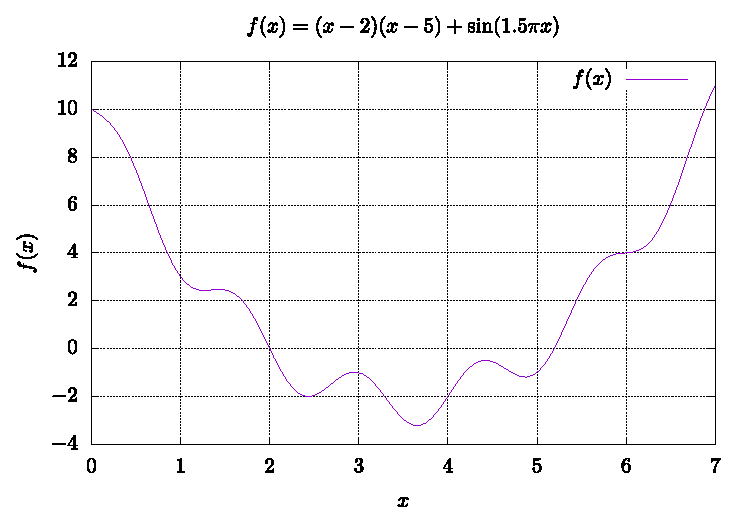
\includegraphics[width=10cm]{grafica1.eps}
\caption{Grafica de la función a analizar.}
\label{fig:g1}
\end{figure}

\begin{equation}
f'(x) = 2x -7 + 1.5 \pi \cos(1.5 \pi x)
\label{ec:derivada}
\end{equation}

Si analizamos detalladamente la  Figura \ref{fig:g2} podemos darnos cuenta que la derivada de la función cruza por cero un total de 7 veces en el intervalo de $[0,7]$, si tratamos de resolver analíticamente este problema nos encontraremos con la problemática que para encontrar los puntos críticos igualando la derivada a cero obtenemos:

\begin{equation}
 2x -7 + 1.5 \pi \cos(1.5 \pi x) = 0
\end{equation} 
la cual es una ecuación que no puede resolverse simbólicamente y es necesario utilizar métodos numéricos, en este caso utilizaremos el método de Newton para encontrar máximos y mínimos, la implementación del algoritmos se muestra en el Código \ref{cod:newton}.

La implementación requiere que calculamos la segunda derivada de la función la cual es:
\begin{equation}
f''(x) = 2 - (1.5 \pi)^{2} \sin(1.5 \pi)
\end{equation}
\begin{figure}[ht!]
\centering
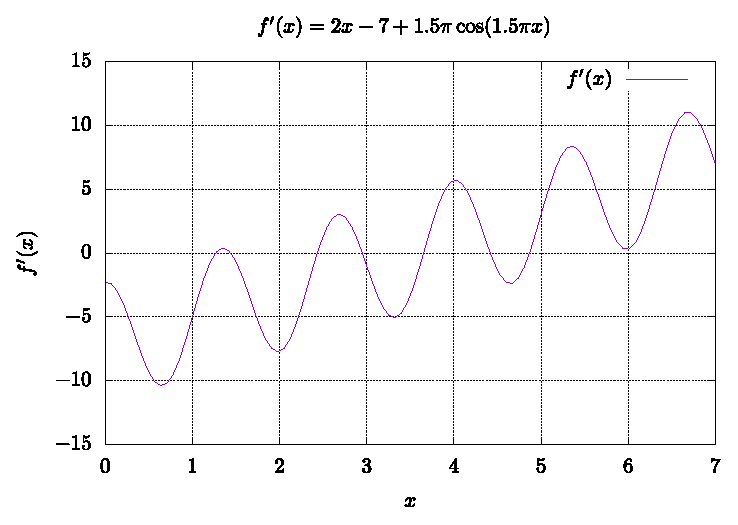
\includegraphics[width=10cm]{grafica2.eps}
\caption{Grafica de la derivada de la función a analizar.}
\label{fig:g2}
\end{figure}
después generamos una solución aleatoria\footnote{La solución aleatoria puede ser entera o flotante, para este ejercicio utilizamos flotante.} (ver Código \ref{cod:random}) de $[0,7]$ que sirva como entrada para el algoritmo de Newton. Para repetir esto 100 veces utilizamos el script en bash que se muestra en el Código \ref{cod:repeat}, el cual escribe un archivo de texto \textbf{datosfloat.txt} que contiene los puntos $x$ donde existe un máximo o un mínimo, sin embargo bajo ciertas entradas el método falló o la solución se encuentra fuera de los rangos deseados, y debido a esto es necesario comprobar cuales fueron las soluciones correctas, esto se hace simplemente ingresando los valores del archivo de texto a la derivada de la función y comprobando que sea menor a cierto umbral, en este caso basta con que sea menor a $1 \times 10^{-4}$, sin embargo optamos por contar el número de ocurrencias de todos los elementos del array para tener más información.

Para procesar los datos utilizamos el Código \ref{cod:analisis}, el cual comprueba que la solución sea valida, después que no sea negativa, calculamos el número de ocurrencias de cada solución y comprobamos si es un máximo o un mínimo .

Del Código \ref{cod:analisis} obtenemos los siguientes resultados:


\begin{table}[!hbp]                                 
		\centering                                       
		\begin{tabular}{ccc}
			\hline                                             
			$x$ & Número de ocurrencias & Max o Min \\                     
			\hline 
			1.264980827648 & 14	& mínimo\\                                            
			1.441085745708 & 15	& máximo\\
			2.433055879795 & 10	& mínimo\\
			2.950004356645 & 4	& máximo\\
			3.652887442162 & 18	& mínimo global\\
			4.418288656759 & 7	& máximo\\
			4.868491681705 & 13	& mínimo\\
			fallos         & 10	& ninguno\\
			$<0$		   & 9	& ninguno\\
			\hline                                             
		\end{tabular}
		\caption{Puntos donde hay un máximo o mínimo.}                                                                                  
	\end{table}	

De los resultados se puede notar que el \textbf{mínimo global} ocurre en $x = 3.652887442162$ y que este ocurre 18 veces, como se hizo 100 veces el experimento esto equivale a un $18\%$.

Algunas notas importantes a tener en cuenta es que para poder ejecutar los archivos .sh hay que cambiar los permisos de ejecución con el comando \textbf{chmod +x filename.sh} y que con cambios muy pequeños a los códigos se pueden hacer 1000 repeticiones y analizar los resultados fácilmente. 

Finalmente podemos concluir que con los códigos que se muestran a continuación se encontraron los los 4 máximos y los 3 mínimos de la función $f(x)$ de los cuales solo uno fue el mínimo global. El método no es muy eficiente y se requieren muchas iteraciones para encontrar la solución correcta sin embargo su complejidad es poca y es en lo que cabe sencillo de implementar.


\newpage
\lstinputlisting[style = PYTHON, caption =  Método de Newton para máximos y mínimos., label = cod:newton]{codigos/newton2.py}

\lstinputlisting[style = PYTHON, caption =  Generar número aleatorio flotante., label = cod:random]{codigos/randomnum.py}

\lstinputlisting[style = BASH, caption = Repeticiones., label = cod:repeat]{codigos/repeat.sh}

\lstinputlisting[style = PYTHON, caption =  Análisis de los datos., label = cod:analisis]{codigos/analisis.py}

\begin{thebibliography}{99}
\bibitem{apuntes} Apuntes y programas de clase Dr. Luis Gerardo de la Fraga.
\end{thebibliography}


\end{document}